\PassOptionsToPackage{dvipsnames}{xcolor}
\documentclass[11pt,aspectratio=169]{beamer}
% metadata
\newcommand{\github}{\href{https://github.com/c-uhs/turnover}{\texttt{https://github.com/c-uhs/turnover}}}
\title
[Risk group turnover in STI/HIV epidemics]
{Risk group turnover in STI/HIV epidemics}
%:\\mechanistic insights from transmission modeling}
\newcommand{\inst}[1]{\enspace\textsuperscript{#1}\thinspace}
\author[\github]
  %[Knight, Wang, Ma, Schwartz, Baral, Mishra]
  {\footnotesize
  Jesse Knight\inst{1},
  Linwei Wang\inst{1},
  Huiting Ma\inst{1},
  Sheree Schwartz\inst{2},
  Stefan Baral\inst{2},
  Sharmistha Mishra\inst{1}
}
\institute{
  \inst{1}MAP Centre for Urban Health Solutions, Unity Health Toronto\\
  \inst{2}Dept.~Epidemiology, Johns Hopkins Bloomberg School of Public Health
}
\newcommand{\logos}{
\begin{tabular}{*{6}{c}}
   
\includegraphics[height=0.75cm,valign=c]{nih-crop}
 & 
\includegraphics[height=0.95cm,valign=c]{cihr}
 & 
\includegraphics[height=0.90cm,valign=c]{jhu}
 & 
\includegraphics[height=0.55cm,valign=c]{map-cuhs}
 & 
\includegraphics[height=0.70cm,valign=c]{smh}
 & 
\includegraphics[height=0.70cm,valign=c]{uoft}
\end{tabular}
}
%\titlegraphic{\vspace{2em}\logos}
\date{2019 July 17}
% temporary paths
\newcommand{\outpath}{../../outputs}
\newcommand{\figpath}{\outpath/paper/sit/figs/}
\newcommand{\tikzpath}{\outpath/tikz/}
\newcommand{\datapath}{\outpath/paper/sit/data/}
% front matter
\makeatletter
\def\abbrfootnote{\gdef\@thefnmark{}\@footnotetext}
\makeatother
% enumerate & itemize
\usepackage{enumitem}
% references
\bibliographystyle{plainnat}
% fixing natbib & hyperref issues
\makeatletter
\def\bibinfo#1{%
  \@ifundefined{bibinfo@X@#1}%
  {\@firstofone}
  {\csname bibinfo@X@#1\endcsname}}
\makeatother
\newcommand*{\doi}[1]{DOI \href{https://doi.org/#1}{\texttt{#1}}}
% maths
\usepackage{bm,amsmath}
\usepackage{xstring}
\newcommand{\tarr}[1]{{\def\arraycolsep{3pt}[\begin{matrix}\StrSubstitute{#1}{,}{&}\end{matrix}]}} % TEMP
\newcommand{\es}{\enspace}
% tables
\usepackage{booktabs,caption,float}
\newcommand{\cellbox}[2]{\parbox[t]{#1}{\linespread{1}\selectfont{#2}}\vspace{3pt}}
% figures
\usepackage{graphicx,subcaption}
\graphicspath{
  {\tikzpath/turnover/}
  {\tikzpath/health/}
  {\tikzpath/tpaf-contexts/}
%  {\tikzpath/variants/}
  {\tikzpath/flows/}
  {\figpath/compare/}
  {\figpath/sensitivity/}
  {\figpath/flows/}
  {\outpath/paper/whatif/asso/figs/compare/}
  {\outpath/paper/whatif/mort/figs/compare/}
  {\outpath/paper/whatif/sirs/figs/compare/}
}
\captionsetup[sub]{size=footnotesize}
% footnotes
\usepackage[hang]{footmisc}
\setlength{\footnotesep}{\baselineskip}
\setlength{\footnotemargin}{1em}
% hyperlink
\usepackage[colorlinks]{hyperref}
% temp formatting
\renewcommand{\floatpagefraction}{0.8}
\interfootnotelinepenalty=10000
% appendix
\newcommand{\initappendix}{
  \appendix
  \numberwithin{figure}{section}
  \numberwithin{table}{section}
  \numberwithin{equation}{section}
  \renewcommand*{\thesection}{\Alph{section}}
}
%\logo{
\includegraphics[width=2cm]{isstdr-full.jpg}}
%%%%%%%%%%%%%%%%%%%%%%%%%%%%%%%%%%%%%%%%%%%%%%%%%%%%%%%%%%%%%%%%%%%%%%%%%%%%%%%%%%%%%%%%%%%%%%%%%%%%
\begin{document}
%%%%%%%%%%%%%%%%%%%%%%%%%%%%%%%%%%%%%%%%%%%%%%%%%%%%%%%%%%%%%%%%%%%%%%%%%%%%%%%%%%%%%%%%%%%%%%%%%%%%
\begin{frame}[noframenumbering]
  \titlepage
\end{frame}
%---------------------------------------------------------------------------------------------------
\begin{frame}[noframenumbering]{}{}
  \vfill
  {\usebeamerfont{frametitle}\usebeamercolor[fg]{frametitle}Disclosures}
  \vfill
  None.
  \vfill\vfill
  {\usebeamerfont{frametitle}\usebeamercolor[fg]{frametitle}Acknowledgements}
  \vfill
  \centering\scalebox{1}{\logos}
\end{frame}
%---------------------------------------------------------------------------------------------------
%\begin{frame}[label=overview]{Overview}
%  \tableofcontents
%\end{frame}
%%%%%%%%%%%%%%%%%%%%%%%%%%%%%%%%%%%%%%%%%%%%%%%%%%%%%%%%%%%%%%%%%%%%%%%%%%%%%%%%%%%%%%%%%%%%%%%%%%%%
\section{Background}
%---------------------------------------------------------------------------------------------------
\begin{frame}{Heterogeneity \& Turnover in Risk}
  \begin{itemize}
    \item \textbf{Core Group Theory (Risk Heterogeneity):}
    \begin{itemize}
      \item Core group is sometimes necessary\,/\,sufficient to sustain an epidemic
      \item Increase $R_0$
      \item Decrease endemic prevalence
    \end{itemize}
    \pause
    \item \textbf{Turnover:}
    \begin{itemize}
      \item Movement of individuals between risk groups (in\,/\,out of the core)
      \item \textsc{aka:} ``episodic risk'', ``migration''
      \item Rarely modelled
    \end{itemize}
  \end{itemize}
\end{frame}
% --------------------------------------------------------------------------------------------------
\begin{frame}{Influence of Turnover in STI Epidemic Models}
  \begin{minipage}{0.62\linewidth}
    \uncover<2->{
    \textbf{Research Questions:}\\[1em]
    Influence of turnover on:}
    \begin{itemize}
      \uncover<3->{\item Equilibrium incidence \& prevalence by risk group}
      \uncover<4->{\item TPAF\,* of core group}
    \end{itemize}
    \vspace*{3em}\footnotesize
    \uncover<5->{
    *\,TPAF: ``transmission population attributable fraction'':\\
    Proportion of cumulative new infections averted\\
    if transmission from that group is stopped}
  \end{minipage}%
  \begin{minipage}{0.38\linewidth}
    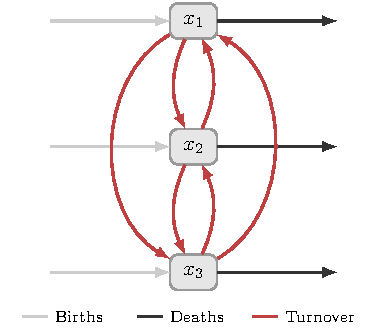
\includegraphics[width=0.9\linewidth]{turnover-simple}
    \pseudocap{Turnover among 3 risk groups}
  \end{minipage}
\end{frame}
%%%%%%%%%%%%%%%%%%%%%%%%%%%%%%%%%%%%%%%%%%%%%%%%%%%%%%%%%%%%%%%%%%%%%%%%%%%%%%%%%%%%%%%%%%%%%%%%%%%%
\section{Methods}
%---------------------------------------------------------------------------------------------------
\begin{frame}{Illustrative Model of STI Transmission}
  \begin{minipage}{0.62\linewidth}
    \begin{itemize}
      \item 1-sex SIR model
      \item 3 risk groups
      \item proportional mixing
      \item turnover rates ensure group sizes don't change
      \item no disease-attributable mortality
    \end{itemize}
    \vspace{1em}
    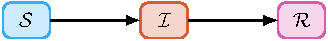
\includegraphics[width=0.5\linewidth]{health-states}
    \pseudocap{Model health states}
  \end{minipage}%
  \begin{minipage}{0.38\linewidth}
    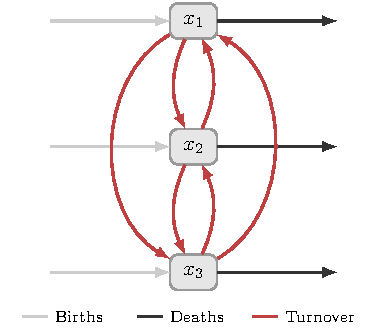
\includegraphics[width=0.9\linewidth]{turnover-simple}
    \pseudocap{Turnover among 3 risk groups}
  \end{minipage}
\end{frame}
%---------------------------------------------------------------------------------------------------
\begin{frame}<1-2>[label=experiment]{Experiments: Influence of Turnover on Model Outputs}
  \begin{enumerate}
    \uncover<1,2,3>{
    \item Equilibrium outputs:
    \begin{itemize}
      \item \parbox{2cm}{\textbf{Vary:}}    Turnover magnitude
      \item \parbox{2cm}{\textbf{Compare:}} a) prevalence, b) incidence (by risk group, at equilibrium)
    \end{itemize}}
    \vspace{1em}
    \uncover<2,4>{
    \item Fitted TPAF:
    \begin{itemize}
      \item \parbox{2cm}{\textbf{Fit:}}     Contact rates, to prevalence: 25\% in core, 5\% in low-risk
      \item \parbox{2cm}{\textbf{Vary:}}    No-turnover vs Turnover
      \item \parbox{2cm}{\textbf{Compare:}} a) Fitted contact rates, b) TPAF of core group
    \end{itemize}}
  \end{enumerate}
\end{frame}
%%%%%%%%%%%%%%%%%%%%%%%%%%%%%%%%%%%%%%%%%%%%%%%%%%%%%%%%%%%%%%%%%%%%%%%%%%%%%%%%%%%%%%%%%%%%%%%%%%%%
\section{Results}
% --------------------------------------------------------------------------------------------------
\againframe<3>[noframenumbering]{experiment}
%---------------------------------------------------------------------------------------------------
\begin{frame}{Turnover decreases core group equilibrium prevalence}
  \visible<2->{
  \begin{minipage}{0.28\linewidth}
    \centering
    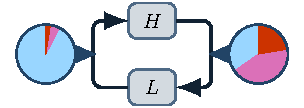
\includegraphics[width=\linewidth]{flows-low}
    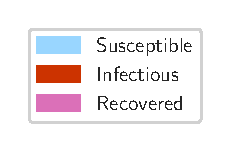
\includegraphics[width=\linewidth]{flows-legend}
    \pseudocap{Low turnover}
    \pseudocap{Risk concentration}
  \end{minipage}}%
  \begin{minipage}{0.44\linewidth}
    \centering
    \includegraphics[width=0.9\linewidth]{{1d-prevalence-high-tau=0.1}.pdf}\\[-0.5em]
    \pseudocap{Core group prevalence vs turnover}
  \end{minipage}%
  \visible<3->{%
  \begin{minipage}{0.28\linewidth}
    \centering
    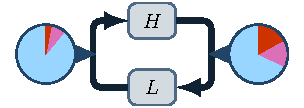
\includegraphics[width=\linewidth]{flows-high}
    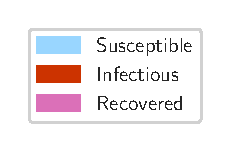
\includegraphics[width=\linewidth]{flows-legend}
    \pseudocap{High turnover}
    \pseudocap{Risk homogenization}
  \end{minipage}}
  \\[1em]
  \uncover<4->{\emph{Turnover causes a net movement of infected: high $\rightarrow$ low risk}}
\end{frame}
% --------------------------------------------------------------------------------------------------
\begin{frame}[t]{Turnover increases low-risk equilibrium prevalence \uncover<2->{\color{C2}\dots at first}}
  \centering
  \begin{minipage}{0.35\linewidth}
    \centering
    \includegraphics[width=\linewidth]{{1d-prevalence-low-extrap-tau=0.1}.pdf}\\[-0.5em]
    \pseudocap{Low-risk prevalence vs turnover}
  \end{minipage}%
  \visible<3->{%
  \begin{minipage}{0.35\linewidth}
    \centering
    \includegraphics[width=\linewidth]{{1d-incidence-all-tau=0.1}.pdf}\\[-0.5em]
    \pseudocap{Overall incidence vs turnover}
  \end{minipage}}%
  \hspace{0.04\linewidth}%
  \visible<4->{%
  \begin{minipage}{0.26\linewidth}
    2 factors of incidence:
    \vspace{0.5em}
    \begin{itemize}
      \item[$\uparrow$] proportion of $\mathcal{I}$
      \item[$\downarrow$] average $C$ among $\mathcal{I}$
    \end{itemize}
    \vspace{3em}
  \end{minipage}}
  \\[1em]\raggedright
  \uncover<5->{\emph{Low turnover: increased exposure
      $\rightarrow$ incidence \& prevalence increase}\\[0.5em]}
  \uncover<6->{\emph{High turnover: homogenization of risk
      $\rightarrow$ incidence \& prevalence decrease}}
\end{frame}
%---------------------------------------------------------------------------------------------------
\againframe<4>[noframenumbering]{experiment}
%---------------------------------------------------------------------------------------------------
\begin{frame}[t]{Turnover makes it harder to observe a high prevalence ratio}
\newcommand{\uin}[2]{\uncover<####1->{\input{data/####2}}}
  \begin{tabular}{llcccccc}
    &&& \multicolumn{2}{c}{\textbf{Before Fitting}} & & \multicolumn{2}{c}{\textbf{After Fitting}}\\
    \cmidrule{4-5}\cmidrule{7-8}
    &&& No turnover & Turnover & & No turnover & Turnover\\[0.5em]
    Contact rate
    & Core     &&       \uin{2}{notu-C-H.txt}    &       \uin{2}{turn-C-H.txt}
               &&       \uin{5}{notu-f-C-H.txt}  &       \uin{5}{turn-f-C-H.txt}  \\
    & Low risk &&       \uin{2}{notu-C-L.txt}    &       \uin{2}{turn-C-L.txt}
               &&       \uin{5}{notu-f-C-L.txt}  &       \uin{5}{turn-f-C-L.txt}  \\
    & Ratio    &&       \uin{2}{notu-C-R.txt}    &       \uin{2}{turn-C-R.txt}
               && \emph{\uin{5}{notu-f-C-R.txt}} & \emph{\uin{5}{turn-f-C-R.txt}} \\[0.5em]
    Prevalence
    & Core     &&       \uin{3}{notu-P-H.txt}    &       \uin{3}{turn-P-H.txt}
               &&       \uin{4}{notu-f-P-H.txt}  &       \uin{4}{turn-f-P-H.txt} \\
    & Low risk &&       \uin{3}{notu-P-L.txt}    &       \uin{3}{turn-P-L.txt}
               &&       \uin{4}{notu-f-P-L.txt}  &       \uin{4}{turn-f-P-L.txt} \\
    & Ratio    && \emph{\uin{3}{notu-P-R.txt}}   & \emph{\uin{3}{turn-P-R.txt}}
               &&       \uin{4}{notu-f-P-R.txt}  &       \uin{4}{turn-f-P-R.txt} \\[0.5em]
  \end{tabular}
  \\
  \uncover<6->{\emph{To observe the same prevalence ratio:\\
      \hspace{1em}Risk heterogeneity must be higher with turnover than without}}\\
  \uncover<7->{\emph{\hspace{1em}(overcome ``homogenizing'' effect of turnover)}}
\end{frame}
% --------------------------------------------------------------------------------------------------
\begin{frame}[t]{After fitting, core group TPAF is higher with turnover than without}
  \begin{minipage}{0.5\linewidth}
    \centering\textbf{Before Fitting}
    \visible<2->{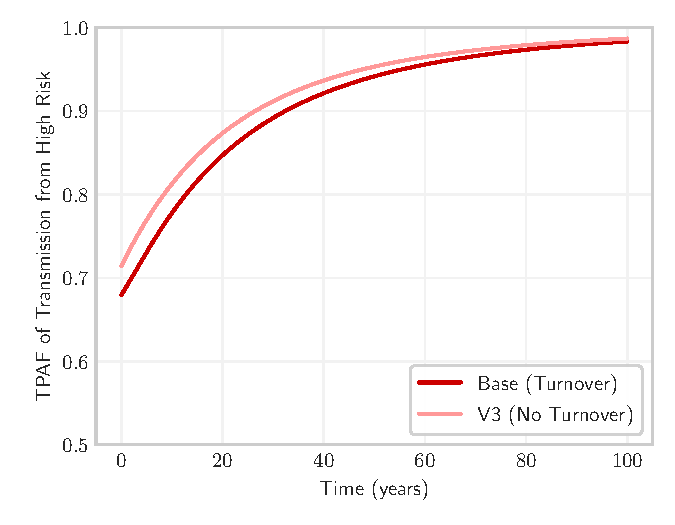
\includegraphics[width=0.7\linewidth]{tpaf-tpaf-high-all-raw}}\\[-0.5em]
    \uncover<3->{\pseudocap{No turnover $\uparrow$ core prevalence}}
    \uncover<4->{\pseudocap{Risk heterogeneity equal ($C$ ratio)}}
  \end{minipage}%
  \begin{minipage}{0.5\linewidth}
    \centering\textbf{After Fitting}
    \visible<5->{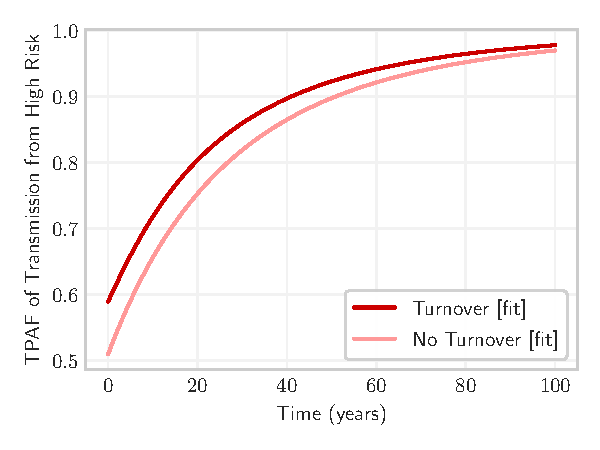
\includegraphics[width=0.7\linewidth]{tpaf-tpaf-high-all-fit}}\\[-0.5em]
    \uncover<6->{\pseudocap{Core prevalence equal}}
    \uncover<7->{\pseudocap{Turnover $\uparrow$ risk heterogeneity ($C$ ratio)}}
  \end{minipage}
  \\[1em]
  \uncover<8->{\emph{TPAF of core group may be underestimated if turnover is not modelled}}
\end{frame}
%%%%%%%%%%%%%%%%%%%%%%%%%%%%%%%%%%%%%%%%%%%%%%%%%%%%%%%%%%%%%%%%%%%%%%%%%%%%%%%%%%%%%%%%%%%%%%%%%%%%
\section{Conclusion}
%---------------------------------------------------------------------------------------------------
\begin{frame}{Implications}{}
  \newcommand{\cnum}[1]{\Large\textcircled{\small{####1}}}
  \begin{enumerate}
    \uncover<2->{
    \item[] Limitations:
    \begin{itemize}
      \item Results shown here conditional on model structure, assumptions, and parameters
    \end{itemize}}
    \vspace{1em}
    \uncover<3->{
    \item[\cnum{1}] \color{C2} Turnover influences equilibrium prevalence \& incidence
    \begin{itemize}
      \item Core prevalence always decreases (before fitting)
      \item Overall effect varies with context
    \end{itemize}}
    \vspace{0.5em}
    \uncover<4->{
    \item[\cnum{2}] \color{C2} TPAF of core group may be underestimated if turnover is not modelled
    \begin{itemize}
      \item Prevalence ratios we observe may be \textit{in spite of} homogenizing effect of turnover
    \end{itemize}}
  \end{enumerate}
\end{frame}
% --------------------------------------------------------------------------------------------------
\begin{frame}[noframenumbering]{Thank you}
  \begin{minipage}{0.45\linewidth}
    \raggedleft
    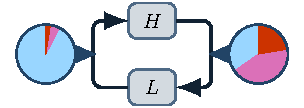
\includegraphics[width=0.6\linewidth]{flows-low}
    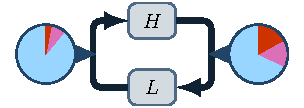
\includegraphics[width=0.6\linewidth]{flows-high}
    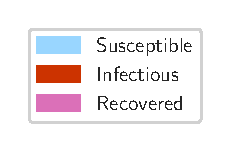
\includegraphics[width=0.6\linewidth]{flows-legend}
  \end{minipage}%
  \hspace{0.1\linewidth}%
  \begin{minipage}{0.45\linewidth}
    \raggedright
    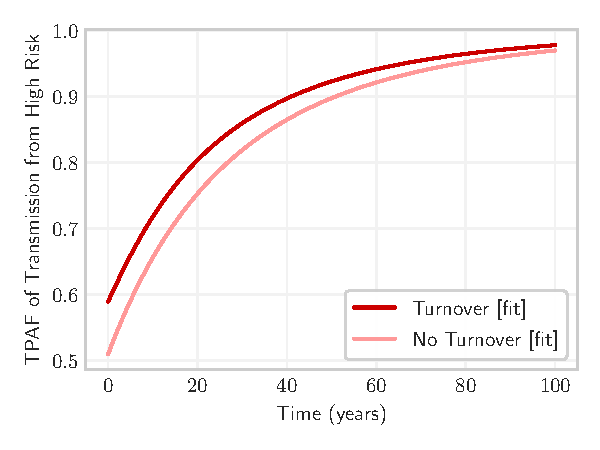
\includegraphics[width=0.8\linewidth]{tpaf-tpaf-high-all-fit}
  \end{minipage}
  \\[2em]\centering\logos
\end{frame}
% --------------------------------------------------------------------------------------------------
\begin{frame}[noframenumbering]{References}
  \printbibliography
\end{frame}
%%%%%%%%%%%%%%%%%%%%%%%%%%%%%%%%%%%%%%%%%%%%%%%%%%%%%%%%%%%%%%%%%%%%%%%%%%%%%%%%%%%%%%%%%%%%%%%%%%%%
\end{document}
%%%%%%%%%%%%%%%%%%%%%%%%%%%%%%%%%%%%%%%%%%%%%%%%%%%%%%%%%%%%%%%%%%%%%%%%%%%%%%%%%%%%%%%%%%%%%%%%%%%%
